\documentclass[12pt,a4paper]{article}

% ─── Page Layout ───────────────────────────────────────────────────────────────
\usepackage[a4paper, margin=0.8in, headheight=14pt]{geometry}

% ─── Fonts (XeLaTeX) ───────────────────────────────────────────────────────────
\usepackage{fontspec}
\usepackage{unicode-math}
\setmainfont{TeX Gyre Pagella}
\setmonofont[Scale=0.88]{TeX Gyre Cursor}
\setmathfont{Latin Modern Math}

% ─── Packages ──────────────────────────────────────────────────────────────────
\usepackage{xcolor}
\usepackage{colortbl}
\usepackage{titlesec}
\usepackage{enumitem}
\usepackage{tabularx}
\usepackage{booktabs}
\usepackage{array}
\usepackage{amsmath}
\usepackage{tikz}
\usetikzlibrary{shapes.geometric, arrows.meta, positioning, calc, fit, decorations.pathreplacing, patterns}
\usepackage{tcolorbox}
\tcbuselibrary{skins, breakable}
\usepackage{hyperref}
\usepackage{fancyhdr}
\usepackage{graphicx}
\usepackage{microtype}
\hyphenpenalty=10000
\exhyphenpenalty=10000
\sloppy
\usepackage{caption}
\usepackage{setspace}
\usepackage{multirow}
\usepackage{tocloft}

% ─── Q&A helper ────────────────────────────────────────────────────────────────
\newcommand{\Q}[1]{\textbf{#1}\par\noindent\ignorespaces}

% ─── Colour Palette ────────────────────────────────────────────────────────────
\definecolor{myred}{RGB}{196,30,58}
\definecolor{mydark}{RGB}{30,30,50}
\definecolor{mygreen}{RGB}{14,120,80}
\definecolor{myteal}{RGB}{0,130,140}
\definecolor{myamber}{RGB}{180,100,0}
\definecolor{mypurple}{RGB}{100,30,160}
\definecolor{mygray}{RGB}{246,247,249}
\definecolor{mgframe}{RGB}{180,185,200}
\definecolor{watermark}{RGB}{145,150,170}
\definecolor{hdrred}{RGB}{250,232,235}
\definecolor{hdrgreen}{RGB}{220,244,233}
\definecolor{hdrteal}{RGB}{220,242,244}
\definecolor{hdramber}{RGB}{253,242,215}
\definecolor{hdrpurple}{RGB}{238,228,255}
\definecolor{hdrgray}{RGB}{238,240,245}
\definecolor{rowalt}{RGB}{250,251,253}

% ─── Section Formatting ────────────────────────────────────────────────────────
\titleformat{\section}
  {\large\bfseries\color{myred}}{\thesection.}{0.5em}{}
  [\vspace{1pt}{\color{myred}\rule{\linewidth}{0.8pt}}]
\titleformat{\subsection}
  {\normalsize\bfseries\color{myteal}}{\thesubsection}{0.5em}{}
\titlespacing*{\section}{0pt}{18pt}{7pt}
\titlespacing*{\subsection}{0pt}{11pt}{4pt}

% ─── Paragraph ─────────────────────────────────────────────────────────────────
\setlength{\parindent}{0pt}
\setlength{\parskip}{4pt}

% ─── TOC Styling ───────────────────────────────────────────────────────────────
\renewcommand{\cfttoctitlefont}{\large\bfseries\color{myred}}
\renewcommand{\cftaftertoctitle}{\par\noindent{\color{myred}\rule{\linewidth}{0.8pt}}}
\setlength{\cftbeforetoctitleskip}{0pt}
\setlength{\cftaftertoctitleskip}{6pt}
\renewcommand{\cftsecfont}{\normalsize\bfseries\color{mydark}}
\renewcommand{\cftsecpagefont}{\normalsize\bfseries\color{mydark}}
\renewcommand{\cftsecleader}{\cftdotfill{\cftdotsep}}
\setlength{\cftbeforesecskip}{7pt}
\renewcommand{\cftsubsecfont}{\small\color{mydark}}
\renewcommand{\cftsubsecpagefont}{\small\color{mydark}}
\setlength{\cftbeforesubsecskip}{3pt}
\setlength{\cftsubsecindent}{1.4em}

% ─── Table helpers ─────────────────────────────────────────────────────────────
\renewcommand{\arraystretch}{1.45}
\setlength{\tabcolsep}{6pt}
\arrayrulecolor{mydark}
\newcolumntype{B}[1]{>{\small\bfseries\raggedright\arraybackslash}m{#1}}
\newcolumntype{Y}{>{\small\raggedright\arraybackslash}X}
\renewcommand{\tabularxcolumn}[1]{m{#1}}

% ─── Header / Footer ───────────────────────────────────────────────────────────
\pagestyle{fancy}
\fancyhf{}
\fancyhead[L]{\small\color{myred}\textbf{EC401}\;\color{mydark}--- Analog Communication}
\fancyhead[R]{\small\color{myteal}\textbf{Module 2 Notes}}
\fancyfoot[C]{\small\color{mydark}\thepage}
\fancyfoot[R]{\small\color{watermark}\textit{\copyright\ Biraj}}
\renewcommand{\headrulewidth}{0.5pt}
\renewcommand{\footrulewidth}{0.3pt}

% ─── Hyperref ──────────────────────────────────────────────────────────────────
\hypersetup{
  colorlinks=true, linkcolor=myteal, urlcolor=myteal,
  pdfauthor={Biraj Sarkar (CGEC)},
  pdftitle={EC401 --- Module 2 Notes: AM and SSB Generation, Detection and Superheterodyne Reception}
}

% ─── tcolorbox styles ──────────────────────────────────────────────────────────
\tcbset{
  tikzbox/.style={
    colback=mygray, colframe=mgframe, boxrule=0.6pt, arc=4pt,
    left=8pt, right=8pt, top=6pt, bottom=6pt,
    colbacktitle=mgframe, coltitle=mydark, fonttitle=\small\bfseries
  },
  defbox/.style={
    colback=hdrgreen, colframe=mygreen, boxrule=0.8pt, arc=4pt,
    left=9pt, right=9pt, top=6pt, bottom=6pt,
    colbacktitle=mygreen, coltitle=white, fonttitle=\small\bfseries
  },
  formulabox/.style={
    colback=hdrteal, colframe=myteal, boxrule=0.8pt, arc=4pt,
    left=9pt, right=9pt, top=7pt, bottom=7pt,
    colbacktitle=myteal, coltitle=white, fonttitle=\small\bfseries
  },
  examplebox/.style={
    colback=hdramber, colframe=myamber, boxrule=0.8pt, arc=4pt,
    left=9pt, right=9pt, top=6pt, bottom=6pt,
    colbacktitle=myamber, coltitle=white, fonttitle=\small\bfseries
  },
  masonbox/.style={
    colback=hdrpurple, colframe=mypurple, boxrule=0.8pt, arc=4pt,
    left=9pt, right=9pt, top=6pt, bottom=6pt,
    colbacktitle=mypurple, coltitle=white, fonttitle=\small\bfseries
  },
  exambox/.style={
    colback=hdrpurple, colframe=mypurple, boxrule=1pt, arc=5pt,
    left=10pt, right=10pt, top=8pt, bottom=8pt,
    colbacktitle=mypurple, coltitle=white, fonttitle=\bfseries,
    breakable, title after break={\textbf{Frequently Asked / Viva Questions (contd.)}}
  }
}
% Allow all boxes to break across pages — prevents footer overflow
\tcbset{breakable}
\tcbset{after={\color{black}}}

% ─── TikZ styles ───────────────────────────────────────────────────────────────
\tikzset{
  block/.style={rectangle, draw=myteal, fill=hdrteal,
    text width=2.4cm, align=center, minimum height=0.95cm,
    font=\small, rounded corners=3pt, line width=0.7pt},
  redblock/.style={rectangle, draw=myred, fill=hdrred,
    text width=2.4cm, align=center, minimum height=0.95cm,
    font=\small, rounded corners=3pt, line width=0.7pt},
  netnode/.style={rectangle, draw=myteal, fill=hdrteal,
    text width=1.5cm, align=center, minimum height=0.8cm,
    font=\small, rounded corners=3pt, line width=0.7pt},
  sumjunc/.style={circle, draw=myamber, fill=hdramber,
    minimum size=0.62cm, font=\small, line width=0.8pt},
  snode/.style={circle, draw=mypurple, fill=hdrpurple,
    minimum size=0.55cm, font=\footnotesize, line width=0.7pt},
  arrow/.style={-Stealth, thick, color=mydark},
  redarrow/.style={-Stealth, thick, color=myred},
  line/.style={thick, color=mydark}
  % ⚠ Do NOT define axis/.style here — conflicts with pgfplots/library keys.
  %   Use inline style instead: \draw[-Stealth, thin, color=mydark]
}

\begin{document}

% ─── Title Page ───────────────────────────────────────────────────────────────
\begin{center}
  {\LARGE\bfseries\color{myred} EC401 --- Analog Communication}\\[5pt]
  {\normalsize\color{mydark} Semester IV \quad$\bullet$\quad 3L:0T:0P \quad$\bullet$\quad 3 Credits}\\[3pt]
  {\normalsize\color{myteal}\textbf{Module 2 Exam Notes: AM and SSB Generation, Detection and Superheterodyne Reception}}\\[3pt]
  {\small\color{mydark} CGEC \;$|$\; B.Tech ECE (2023--27) \;$|$\; \textit{Biraj Sarkar}}
\end{center}
\vspace{2pt}
\noindent{\color{myred}\rule{\linewidth}{1.5pt}}
\vspace{2pt}

\hypersetup{linkcolor=mydark}
\tableofcontents
\hypersetup{linkcolor=myteal}
\newpage

\section{Generation and Detection of Amplitude Modulation}
\subsection{Gated Modulator}
\begin{tcolorbox}[defbox, title={Carrier-Controlled Switching}]
A carrier-frequency switch gates a DC-biased message $u(t)=B+m(t)$. A band-pass filter (BPF) centred at $f_c$ selects the RF fundamental and its sidebands. For ideal half-duty gating $g(t)=1$ when $\cos(2\pi f_ct)>0$ and zero otherwise:
\[
\begin{aligned}
 g(t)&=\frac12+\frac{2}{\pi}\left[
 \cos(2\pi f_ct)-\frac13\cos(6\pi f_ct)+\cdots\right],\\
 v(t)&=[B+m(t)]g(t),\\
 s(t)&=\frac{2B}{\pi}\left[1+\frac{m(t)}{B}\right]\cos(2\pi f_ct).
\end{aligned}
\]
The BPF rejects baseband and harmonics. With $B=0$, the same ideal switch and filter produce DSB-SC from a zero-mean message. Real switching requires adequate carrier drive and filtering.
\end{tcolorbox}

\begin{tcolorbox}[tikzbox, unbreakable, title={Gated and Square-Law AM Generation}]
\centering
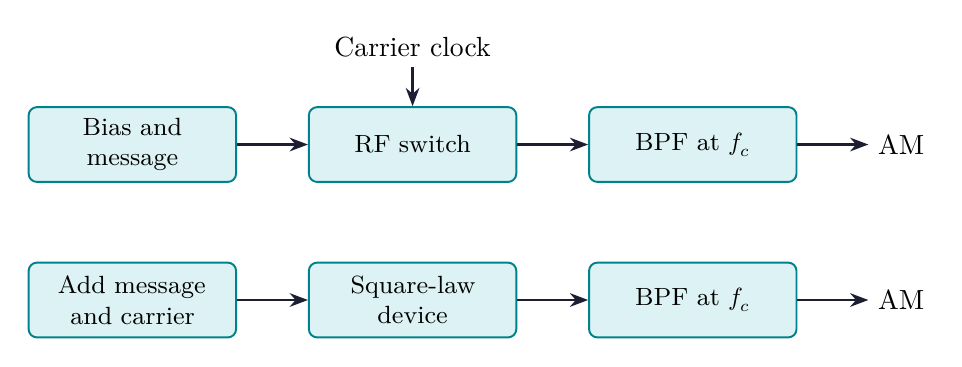
\begin{tikzpicture}[node distance=9mm]
  \node[block] (bias) {Bias and message};
  \node[block,right=of bias] (gate) {RF switch};
  \node[block,right=of gate] (bpf) {BPF at $f_c$};
  \node[right=9mm of bpf] (out) {AM};
  \draw[arrow] (bias)--(gate);
  \draw[arrow] (gate)--(bpf);
  \draw[arrow] (bpf)--(out);
  \node[above=5mm of gate] (osc) {Carrier clock};
  \draw[arrow] (osc)--(gate);
  \node[block,below=10mm of bias] (sum) {Add message and carrier};
  \node[block,right=of sum] (sq) {Square-law device};
  \node[block,right=of sq] (sel) {BPF at $f_c$};
  \node[right=9mm of sel] (out2) {AM};
  \draw[arrow] (sum)--(sq);
  \draw[arrow] (sq)--(sel);
  \draw[arrow] (sel)--(out2);
\end{tikzpicture}\par
\end{tcolorbox}

\subsection{Square-Law Modulator}
\begin{tcolorbox}[defbox, title={Square-Law Modulator}]
A \textbf{square-law modulator} uses the quadratic response of a nonlinear device to mix a message with a carrier. The squared term produces the message--carrier product, and a band-pass filter selects the carrier and its sidebands.
\end{tcolorbox}

For a weakly nonlinear device $v_o=a_1v_i+a_2v_i^2$, let $v_i=m(t)+A\cos\omega_ct$. The coefficient $a_2$ has units $\mathrm{V^{-1}}$ for voltage in and out. Expand before filtering:
\[
\begin{aligned}
 v_o &= a_1m+a_1 A\cos\omega_ct+a_2m^2\\
     &\quad+2a_2Am\cos\omega_ct+a_2A^2\cos^2\omega_ct,\\
 s(t)&=a_1A\cos\omega_ct+2a_2Am(t)\cos\omega_ct\\
     &=a_1A\left[1+\frac{2a_2}{a_1}m(t)\right]\cos\omega_ct.
\end{aligned}
\]
The BPF removes $a_1m$, $a_2m^2$, DC and $2f_c$. This model assumes weak nonlinearity and a carrier well separated from the baseband harmonics.

\subsection{Balanced Modulator}
Two matched AM branches receive opposite message voltages and a common carrier. Subtracting their outputs cancels the carrier:
\[
\begin{aligned}
 u_+&=A_c(1+k_am)\cos\omega_ct,\quad
 u_-=A_c(1-k_am)\cos\omega_ct,\\
 s_D&=u_+-u_-\\
    &=2A_ck_a m(t)\cos\omega_ct.
\end{aligned}
\]
A transformer-coupled diode ring can implement balanced switching by reversing message polarity at the carrier rate. Mismatch leaves residual carrier. Balance and filtering set suppression in practice.

\begin{tcolorbox}[examplebox, title={Square-Law Modulator with a Specified Carrier and Tone}]
Let $v_o=2v_i+0.2v_i^2$, with the quadratic coefficient in $\mathrm{V^{-1}}$. The input combines a $4\,\mathrm V$ peak carrier and a $1.5\,\mathrm V$ peak message tone.
\[
\begin{aligned}
 A_{c,\rm out} &= a_1A=2(4)=8\,\mathrm V,\\
 k_a &= \frac{2a_2}{a_1}=\frac{2(0.2)}{2}=0.2\,\mathrm{V^{-1}},\\
 \mu&=k_aA_m=(0.2)(1.5)=0.30,\\
 A_{\rm USB}=A_{\rm LSB}&=\frac{\mu A_{c,\rm out}}2=1.2\,\mathrm V.
\end{aligned}
\]
The RF filter must pass both sidebands of the selected carrier and reject the terms around DC and $2f_c$. The result follows from the quadratic model. A practical circuit has higher-order terms and must limit its input swing.
\end{tcolorbox}

\subsection{Carrier Leakage in a Balanced Modulator}
If the lower branch has gain $g$ relative to the upper branch, the subtractor output is
\[
\begin{aligned}
 s(t) &= A_c[(1+k_am)-g(1-k_am)]\cos\omega_ct\\
      &= A_c(1-g)\cos\omega_ct
        +A_c(1+g)k_am(t)\cos\omega_ct.
\end{aligned}
\]
The first term is carrier leakage. For $g=0.98$ and $k_aA_m=0.5$, the leakage amplitude is $0.02A_c$. Each sideband has amplitude $(1.98)(0.5)A_c/2=0.495A_c$. The carrier is about $20\log_{10}(0.495/0.02)=27.9\,\mathrm{dB}$ below either sideband. Matching bias and gain reduces the leakage. Carrier suppression and sideband selection are separate design steps.

\section{Generation of Single Sideband}
\subsection{Filter Method}
Generate DSB-SC, pass only the desired sideband with a sharp BPF, and translate the retained band to its final channel if required. A message with lowest nonzero frequency $f_{\min}$ gives a gap of $2f_{\min}$ between the occupied bands. Little or no gap makes the filter difficult. Speech transmitters can limit low-frequency audio and first form SSB at a convenient IF.

\subsection{Phase-Shift Method}
Use a broadband $90^\circ$ message shifter to generate $\widehat m(t)$ and a carrier quadrature shifter to generate $\sin\omega_ct$. The balanced products are $m\cos\omega_ct$ and $\widehat m\sin\omega_ct$. Subtract for USB and add for LSB with this choice of phase:
\[
\begin{aligned}
 \cos\omega_mt\cos\omega_ct-\sin\omega_mt\sin\omega_ct
   &=\cos[(\omega_c+\omega_m)t],\\
 \cos\omega_mt\cos\omega_ct+\sin\omega_mt\sin\omega_ct
   &=\cos[(\omega_c-\omega_m)t].
\end{aligned}
\]
Gain or phase errors prevent complete cancellation. Maintaining a broadband quadrature shift is the main limitation.

\subsection{Third Method (Weaver)}
Weaver replaces the broadband audio phase shifter with two quadrature mixing stages and matched low-pass filters (LPFs). For an occupied message band $f_a$ to $f_b$, choose $f_0=(f_a+f_b)/2$. The first LPFs pass difference frequencies up to $(f_b-f_a)/2$. For a tone of peak $A_m$, let $\delta=2\pi(f_m-f_0)$:
\[
 I=\operatorname{LPF}[m\cos(2\pi f_0t)]
   =\frac{A_m}{2}\cos\delta t,\qquad
 Q=-\operatorname{LPF}[m\sin(2\pi f_0t)]
   =\frac{A_m}{2}\sin\delta t.
\]
The second stage combines $I\cos\omega_2t-Q\sin\omega_2t$ for USB with $f_2=f_c+f_0$, giving $f_2+(f_m-f_0)=f_c+f_m$. The sum gives the LSB if the second oscillator is set to $f_c-f_0$. Matched LPFs and quadrature oscillator accuracy determine image rejection.

\begin{tcolorbox}[tikzbox, unbreakable, title={Weaver Upper Sideband Signal Paths}]
\centering
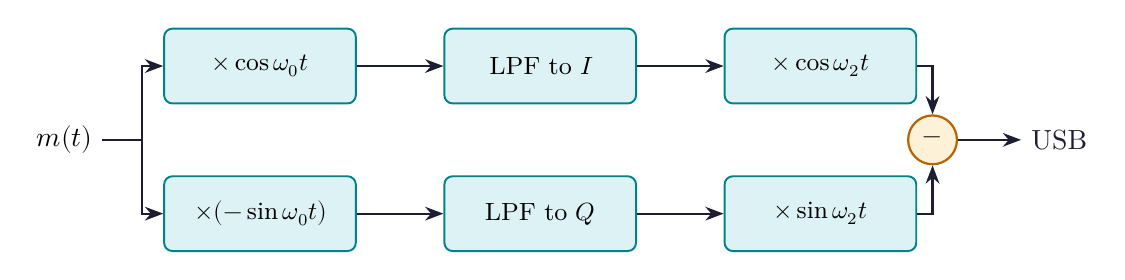
\begin{tikzpicture}[sblock/.style={block,text width=2.2cm},node distance=11mm]
  \node[sblock] (ic) {$\times\cos\omega_0t$};
  \node[sblock,below=9mm of ic] (qs) {$\times(-\sin\omega_0t)$};
  \node[sblock,right=of ic] (il) {LPF to $I$};
  \node[sblock,right=of qs] (ql) {LPF to $Q$};
  \node[sblock,right=of il] (mixi) {$\times\cos\omega_2t$};
  \node[sblock,right=of ql] (mixq) {$\times\sin\omega_2t$};
  \coordinate (mid) at ($(ic.center)!0.5!(qs.center)$);
  \node[left=20mm of mid] (in) {$m(t)$};
  \node[sumjunc,right=11mm of $(mixi.center)!0.5!(mixq.center)$] (sub) {$-$};
  \draw[arrow] (in.east)--++(5mm,0) |- (ic.west);
  \draw[arrow] (in.east)--++(5mm,0) |- (qs.west);
  \draw[arrow] (ic)--(il);
  \draw[arrow] (qs)--(ql);
  \draw[arrow] (il)--(mixi);
  \draw[arrow] (ql)--(mixq);
  \draw[arrow] (mixi.east)-| (sub.north);
  \draw[arrow] (mixq.east)-| (sub.south);
  \draw[arrow] (sub.east)--++(8mm,0) node[right] {USB};
\end{tikzpicture}\par
\end{tcolorbox}

\begin{tcolorbox}[examplebox, title={Weaver Frequency Plan for a Speech Channel}]
A voice channel spans $300$ to $2700\,\mathrm{Hz}$. Form USB on a $500\,\mathrm{kHz}$ nominal carrier.
\[
\begin{aligned}
 f_0&=\frac{300+2700}{2}=1500\,\mathrm{Hz},\\
 W_{\rm LP}&=\frac{2700-300}{2}=1200\,\mathrm{Hz},\\
 f_2&=f_c+f_0=501.5\,\mathrm{kHz}.
\end{aligned}
\]
After quadrature mixing and subtraction, the RF frequencies are $f_2+(f_m-f_0)$. A $900\,\mathrm{Hz}$ tone produces $500.9\,\mathrm{kHz}$, whereas $2400\,\mathrm{Hz}$ produces $502.4\,\mathrm{kHz}$. The occupied band is $500.3$--$502.7\,\mathrm{kHz}$. The negative difference frequency for $900\,\mathrm{Hz}$ is preserved by the quadrature paths.
\end{tcolorbox}

\subsection{Effect of Phase Error in the Phase-Shift Method}
For matched gains and an error $\delta$ in the relative quadrature phase, the two branch contributions at the wanted line add as $1+e^{j\delta}$. The unwanted line receives the difference $1-e^{j\delta}$. The amplitude leakage ratio is
\[
 \left|\frac{1-e^{j\delta}}{1+e^{j\delta}}\right|
   =\left|\tan\frac{\delta}{2}\right|.
\]
At a $5^\circ$ phase error, leakage is about $0.0437$ times the wanted line amplitude, or about $27.2\,\mathrm{dB}$ below it. A phase shifter that is accurate only at one audio frequency will give different rejection over the message band.

\section{Demodulation of Linear Modulation}
\subsection{AM Envelope Detector}
\begin{tcolorbox}[defbox, title={Diode Peak Detector}]
A diode charges $C$ near RF peaks, then blocks as the input falls. Between peaks, $C$ discharges through the load $R$. The smoothed voltage follows the envelope. A coupling capacitor or DC removal stage then recovers the audio. A large carrier, no envelope folding and a suitable $RC$ are required.
\end{tcolorbox}

\begin{tcolorbox}[tikzbox, unbreakable, title={Diode Envelope Detector Circuit}]
\centering
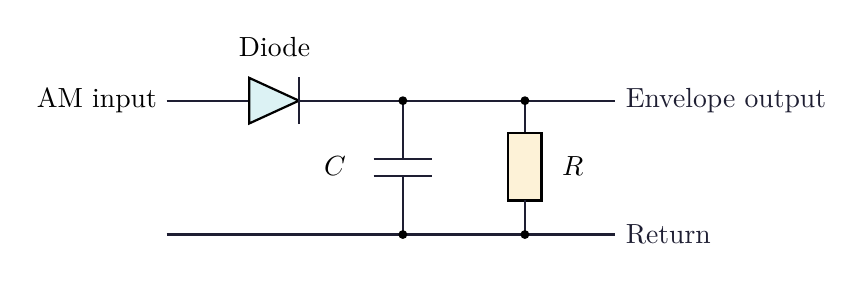
\begin{tikzpicture}[x=1cm,y=0.85cm]
  \node[left] at (0,2) {AM input};
  \draw[line] (0,2)--(1.05,2);
  \draw[fill=hdrteal,thick] (1.05,1.66)--(1.05,2.34)--(1.68,2)--cycle;
  \draw[line] (1.68,1.65)--(1.68,2.35);
  \draw[line] (1.68,2)--(5.7,2) node[right] {Envelope output};
  \node[above=4pt] at (1.37,2.35) {Diode};
  \draw[line] (0,0)--(5.7,0) node[right] {Return};
  \draw[line] (3,2)--(3,1.13);
  \draw[line] (2.63,1.13)--(3.37,1.13);
  \draw[line] (2.63,0.88)--(3.37,0.88);
  \draw[line] (3,0.88)--(3,0);
  \node[left=7pt] at (2.63,1.02) {$C$};
  \draw[line] (4.55,2)--(4.55,1.52);
  \draw[thick,fill=hdramber] (4.34,0.51) rectangle (4.76,1.52);
  \draw[line] (4.55,0.51)--(4.55,0);
  \node[right=4pt] at (4.76,1.02) {$R$};
  \foreach \x in {3,4.55}{\fill (\x,2) circle (1.6pt); \fill (\x,0) circle (1.6pt);}
\end{tikzpicture}\par
\end{tcolorbox}

Choose $RC$ long compared with the carrier period and short enough to follow the steepest envelope fall. Too short gives carrier ripple. Too long gives diagonal clipping. If $E(t)$ is the positive envelope, the ideal discharge slope just after a peak is $-E/RC$. On a falling part the discharge must be at least as steep:
\[
 RC\le \min_{\dot E<0}\frac{E(t)}{|\dot E(t)|}.
\]
With $E=A_c(1+\mu\cos\omega_mt)$, this ratio on the falling half-cycle is $(1+\mu\cos\theta)/(\mu\omega_m\sin\theta)$. Differentiating with respect to $\theta$ gives a stationary point at $\cos\theta=-\mu$. Therefore, for $0<\mu<1$,
\[
 \frac{1}{f_c}\ll RC
 \ \lesssim\ \frac{\sqrt{1-\mu^2}}{\mu\,2\pi f_m}.
\]
Real diode drop, source resistance and loading affect the actual design.

\begin{tcolorbox}[examplebox, title={Select a Detector Time Constant}]
Let $f_c=1\,\mathrm{MHz}$, $f_m=5\,\mathrm{kHz}$ and $\mu=0.6$.
\[
\begin{aligned}
 T_c &=1\,\mu\mathrm{s},\\
 RC_{\max}&=\frac{\sqrt{1-0.6^2}}{0.6(2\pi)(5000)}
            \approx42.4\,\mu\mathrm{s}.
\end{aligned}
\]
A starting choice is $R=10\,\mathrm{k}\Omega$ and $C=1.5\,\mathrm{nF}$, giving $RC=15\,\mu\mathrm{s}$. Check ripple and clipping at the worst specified modulation in the actual circuit.
\end{tcolorbox}

\subsection{Synchronous Detection and Mismatch}
Multiply $A_cm(t)\cos(2\pi f_ct)$ by $2\cos[2\pi(f_c+\Delta f)t+\phi]$ and low-pass filter:
\[
\begin{aligned}
 v(t)&=A_cm(t)\cos(2\pi\Delta ft+\phi)\\
     &\quad+A_cm(t)\cos[2\pi(2f_c+\Delta f)t+\phi],\\
 v_{\rm LP}(t)&=A_cm(t)\cos(2\pi\Delta ft+\phi).
\end{aligned}
\]
With only phase error, recovered amplitude scales by $\cos\phi$. At $90^\circ$ it vanishes. With frequency error the gain oscillates, causing beats and sign changes. A transmitted pilot can drive a carrier-recovery PLL. For DSB-SC without a pilot, a Costas loop or squaring loop can regenerate the reference. A recovered reference may retain a $180^\circ$ ambiguity, resolved by a known pilot or polarity reference. If RF filtering or the LPF removes part of a mismatch-shifted spectrum, the resulting waveform is additionally distorted.

\subsection{Carrier Recovery for DSB-SC: Squaring Loop and Costas Loop}
Because DSB-SC suppresses the carrier component completely, a coherent receiver must synthesize the carrier frequency and phase directly from the received sidebands. Two canonical circuits accomplish this:

\paragraph{1. Squaring Loop}
Passing $s(t)=A_cm(t)\cos(\omega_ct+\theta)$ through a square-law nonlinearity gives:
\[
s^2(t)=A_c^2m^2(t)\cos^2(\omega_ct+\theta)=\frac{1}{2}A_c^2m^2(t)\left[1+\cos(2\omega_ct+2\theta)\right].
\]
Since $m^2(t)\ge 0$ for all $t$, its expected value $\overline{m^2(t)}=P_m$ is strictly non-zero. A narrow bandpass filter (or PLL) centered at $2f_c$ extracts this discrete harmonic:
\[
v_{2f_c}(t)=\frac{1}{2}A_c^2P_m\cos(2\omega_ct+2\theta).
\]
Passing this signal through a frequency divider by two produces $\cos(\omega_ct+\theta)$ or $-\cos(\omega_ct+\theta)$, providing the coherent local reference with a $180^\circ$ phase ambiguity.

\paragraph{2. Costas Loop}
The Costas loop avoids RF frequency squaring by detecting the phase error directly at baseband through In-phase ($I$) and Quadrature ($Q$) channels:

\begin{tcolorbox}[tikzbox, unbreakable, title={Costas Loop Architecture for Coherent Carrier Recovery}]
\centering
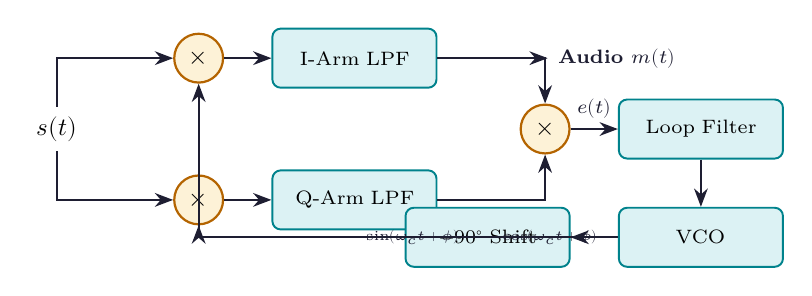
\begin{tikzpicture}[node distance=6mm, sblock/.style={block, text width=1.85cm, minimum height=0.75cm, font=\scriptsize}]
  \node (in) at (0,1.2) {\small $s(t)$};
  \node[sumjunc] (m1) at (1.8,2.1) {$\times$};
  \node[sumjunc] (m2) at (1.8,0.3) {$\times$};
  \node[sblock, right=of m1] (lpf1) {I-Arm LPF};
  \node[sblock, right=of m2] (lpf2) {Q-Arm LPF};
  \node[sumjunc] (m3) at (6.2,1.2) {$\times$};
  \node[sblock, right=of m3] (lf) {Loop Filter};
  \node[sblock, below=of lf] (vco) {VCO};
  \node[sblock, left=of vco] (ps) {$-90^\circ$ Shift};

  \draw[arrow] (in) |- (m1);
  \draw[arrow] (in) |- (m2);
  \draw[arrow] (m1) -- (lpf1);
  \draw[arrow] (m2) -- (lpf2);
  \draw[arrow] (lpf1.east) -| (m3.north);
  \draw[arrow] (lpf2.east) -| (m3.south);
  \draw[arrow] (m3) -- node[above] {\scriptsize $e(t)$} (lf);
  \draw[arrow] (lf) -- (vco);
  \draw[arrow] (vco) -- (ps);
  \draw[arrow] (vco.west) -| (m1.south) node[pos=0.15, right] {\tiny $\cos(\omega_c t+\phi)$};
  \draw[arrow] (ps.west) -| (m2.south) node[pos=0.15, right] {\tiny $-\sin(\omega_c t+\phi)$};
  \draw[arrow] (lpf1.east) -- ++(1.4,0) node[right] {\scriptsize \textbf{Audio $m(t)$}};
\end{tikzpicture}\par
\small When $\phi$ is small, the I-arm LPF yields $v_I(t)\approx\frac{A_c}{2}m(t)$ and the Q-arm LPF yields $v_Q(t)\approx\frac{A_c}{2}m(t)\phi$. Their product is $e(t)\approx\frac{A_c^2}{4}m^2(t)\phi$. Since $m^2(t)>0$, the loop filter integrates a DC error voltage strictly proportional to $\phi$, steering the VCO until $\phi\to 0$.
\end{tcolorbox}

\begin{tcolorbox}[examplebox, title={Frequency and Phase Error in a Coherent Receiver}]
For $m(t)=\cos(2\pi\,1000t)$, unit RF scale, and LO frequency offset $20\,\mathrm{Hz}$ with zero initial phase error, the detector yields
\[
 \begin{aligned}
 v_o(t)&=\cos(2\pi\,1000t)\cos(2\pi\,20t)\\
       &=\tfrac12\cos(2\pi\,1020t)+\tfrac12\cos(2\pi\,980t).
 \end{aligned}
\]
The two components bracket the original tone. With frequency lock restored but a constant $60^\circ$ phase error, the output instead becomes a single $1\,\mathrm{kHz}$ tone at half amplitude. Carrier phase and frequency recovery address different errors.
\end{tcolorbox}

\section{Superheterodyne Receiver}
Changing stations retunes the front end and local oscillator together so the wanted signal reaches the same intermediate-frequency filter.

\begin{tcolorbox}[defbox, title={Mix to a Fixed Intermediate Frequency}]
A tunable RF front end selects a station. The mixer shifts it to a fixed intermediate frequency (IF), where selectivity and gain are easier to implement. For the difference product,
\[
 f_{\rm IF}=|f_{\rm RF}-f_{\rm LO}|.
\]
The unwanted image lies on the opposite side of the LO from the desired RF. Both yield the same IF. The RF preselector must attenuate the image before mixing.
\end{tcolorbox}

\begin{tcolorbox}[tikzbox, unbreakable, title={Superheterodyne Receiver with RF Preselection and IF Filtering}]
\centering
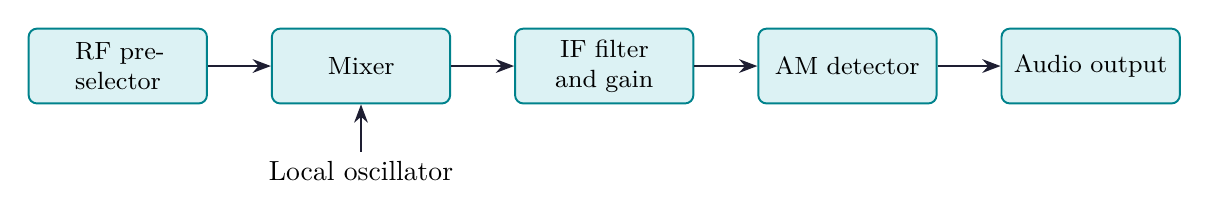
\begin{tikzpicture}[sblock/.style={block,text width=2.03cm},node distance=8mm]
  \node[sblock] (rf) {RF preselector};
  \node[sblock,right=of rf] (mix) {Mixer};
  \node[sblock,right=of mix] (if) {IF filter and gain};
  \node[sblock,right=of if] (det) {AM detector};
  \node[sblock,right=of det] (audio) {Audio output};
  \node[below=6mm of mix] (lo) {Local oscillator};
  \draw[arrow] (rf)--(mix);
  \draw[arrow] (mix)--(if);
  \draw[arrow] (if)--(det);
  \draw[arrow] (det)--(audio);
  \draw[arrow] (lo)--(mix);
\end{tikzpicture}\par
\end{tcolorbox}

\begin{tcolorbox}[formulabox, title={High-Side and Low-Side Injection}]
\[
\begin{aligned}
 \text{High-side:}\quad
 f_{\rm LO}&=f_{\rm RF}+f_{\rm IF}, & f_{\rm im}&=f_{\rm RF}+2f_{\rm IF},\\
 \text{Low-side:}\quad
 f_{\rm LO}&=f_{\rm RF}-f_{\rm IF}, & f_{\rm im}&=f_{\rm RF}-2f_{\rm IF}.
\end{aligned}
\]
The low-side image expression here assumes a positive physical RF image in the difference-mixing case. A larger IF separates the image further, while a lower IF can simplify sharp selectivity. Dual conversion can combine these benefits.
\end{tcolorbox}

\subsection{Receiver Selectivity before and after Mixing}
In high-side injection the wanted RF and the image lie below and above the LO, respectively. Taking the difference at the mixer maps both to the same IF. Increasing IF increases the $2f_{\rm IF}$ image separation. Tightening the RF preselector also improves image rejection, but it must still pass both wanted AM sidebands. The fixed IF filter sets adjacent-channel selectivity after conversion. Automatic gain control adjusts receiver gain as station strength varies.

\begin{tcolorbox}[tikzbox, unbreakable, title={Two RF Inputs Can Produce the Same Intermediate Frequency}]
\centering
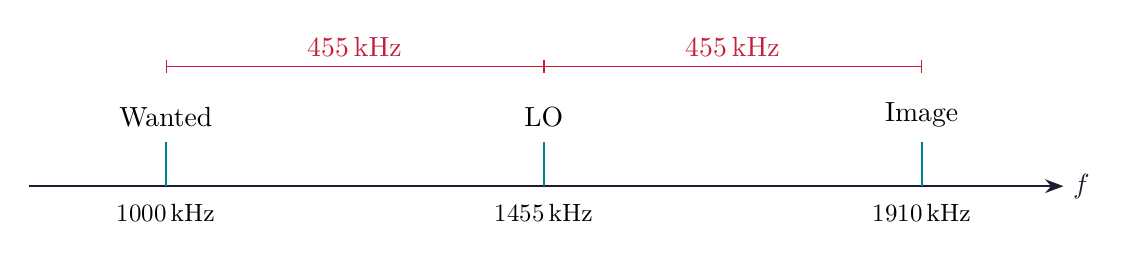
\begin{tikzpicture}[x=1.2cm,y=1cm]
 \draw[arrow] (-0.45,0)--(10.5,0) node[right] {$f$};
 \foreach \x/\f/\lab in {1/1000/Wanted,5/1455/LO,9/1910/Image}{
   \draw[myteal,thick] (\x,0)--(\x,0.56);
   \node[above=2pt] at (\x,0.56) {\lab};
   \node[below=3pt] at (\x,0) {\small $\f\,\mathrm{kHz}$};
 }
 \draw[|-|,myred] (1,1.52)--(5,1.52) node[midway,above] {$455\,\mathrm{kHz}$};
 \draw[|-|,myred] (5,1.52)--(9,1.52) node[midway,above] {$455\,\mathrm{kHz}$};
\end{tikzpicture}\par
\end{tcolorbox}

\begin{tcolorbox}[examplebox, title={Compute LO and Image Frequencies}]
For $f_{\rm RF}=1000\,\mathrm{kHz}$, $f_{\rm IF}=455\,\mathrm{kHz}$ and high-side injection,
\[
\begin{aligned}
 f_{\rm LO}&=1000+455=1455\,\mathrm{kHz},\\
 f_{\rm im}&=1455+455=1910\,\mathrm{kHz},\\
 |1910-1455|&=|1000-1455|=455\,\mathrm{kHz}.
\end{aligned}
\]
With low-side injection the LO is at $545\,\mathrm{kHz}$ and the corresponding image is at $90\,\mathrm{kHz}$. Both cases place the image $910\,\mathrm{kHz}$ from the desired station.
\end{tcolorbox}

\begin{tcolorbox}[examplebox, title={Calculate Image Rejection of a Single Tuned RF Stage}]
For an ideal single tuned preselector at $f_s$ with loaded quality factor $Q$, the normalized off-tune voltage gain is
\[
 \frac{|H(f)|}{|H(f_s)|}
 =\frac{1}{\sqrt{1+Q^2(f/f_s-f_s/f)^2}} .
\]
This form follows from the conductance and susceptance of a parallel RLC circuit. At $f_s=1\,\mathrm{MHz}$ with $Q=50$, compare high-side injection at two IFs:
\[
\begin{aligned}
 f_{\rm IF}=455\,\mathrm{kHz}:\quad f_{\rm im}&=1.910\,\mathrm{MHz},
 & |H(f_{\rm im})|/|H(f_s)|&\approx0.0144,\\[2pt]
 f_{\rm IF}=100\,\mathrm{kHz}:\quad f_{\rm im}&=1.200\,\mathrm{MHz},
 & |H(f_{\rm im})|/|H(f_s)|&\approx0.0545.
\end{aligned}
\]
The reductions are approximately $36.8$ and $25.3\,\mathrm{dB}$ respectively for equal antenna input voltages. A higher IF moves the image farther down the preselector response. The loaded bandwidth near resonance is about $f_s/Q=20\,\mathrm{kHz}$, so this example can still pass a $10\,\mathrm{kHz}$ wide AM channel.
\end{tcolorbox}

\newpage
\begin{center}
  {\large\bfseries\color{myred} Quick Revision --- Module 2}\\[3pt]
  {\small\color{mydark} AM and SSB Generation, Detection and Superheterodyne Reception $|$ EC401}
\end{center}
\noindent{\color{myred}\rule{\linewidth}{1.2pt}}
\par\vspace{4pt}

\begin{tcolorbox}[formulabox, title={Key Formulas at a Glance}]
\renewcommand{\arraystretch}{1.35}
\noindent\begin{tabularx}{\linewidth}{B{4.4cm} Y}
Gated AM & $\frac{2}{\pi}[B+m(t)]\cos(2\pi f_ct)$ \\[4pt]
Square-law AM & $k_a=2a_2/a_1$ after BPF \\[4pt]
Balanced output & $s_D=2A_ck_am(t)\cos\omega_ct$ \\[4pt]
Phase-shift SSB & $m\cos\omega_ct\mp\widehat m\sin\omega_ct$ \\[4pt]
Envelope detector & $1/f_c\ll RC\lesssim\sqrt{1-\mu^2}/(\mu\,2\pi f_m)$ \\[4pt]
Coherent mismatch & $v_{\rm LP}=A_cm(t)\cos(2\pi\Delta ft+\phi)$ \\[4pt]
IF and image & $f_{\rm IF}=|f_{\rm RF}-f_{\rm LO}|$ \newline $f_{\rm im}=f_{\rm RF}\pm2f_{\rm IF}$ for the indicated injection \\[4pt]
\end{tabularx}\par
\end{tcolorbox}

\begin{tcolorbox}[defbox, title={One-Line Definitions}, title after break={One-Line Definitions (contd.)}]
\begin{itemize}[leftmargin=*, itemsep=3pt, topsep=0pt]
  \item \textbf{Intermediate frequency (IF).} The fixed frequency to which a superheterodyne receiver converts the selected signal before filtering and demodulation.
  \item \textbf{Balanced modulator.} A modulator that multiplies the message by the carrier and cancels the separate carrier component, producing a double-sideband suppressed-carrier signal.
  \item \textbf{Diagonal clipping.} Envelope-detector distortion that occurs when its capacitor discharges too slowly to follow a falling AM envelope.
  \item \textbf{Image.} An unwanted radio-frequency signal that the mixer converts to the same intermediate frequency as the desired signal.
  \item \textbf{Coherent detection.} Recovery of a message by multiplying the received signal by a local reference matched to the transmitted carrier in frequency and phase.
\end{itemize}
\end{tcolorbox}

\begin{tcolorbox}[exambox, title={Frequently Asked / Viva Questions}]
\begin{enumerate}[topsep=0pt, label=\textbf{Q\arabic*.}, itemsep=5pt]
  \item \Q{What selects the fundamental in a gated modulator?}
    An RF BPF at the switching frequency rejects the baseband and higher harmonic groups.
  \item \Q{Which square-law term creates sidebands?}
    The cross-product $2a_2Am\cos\omega_ct$.
  \item \Q{What causes residual carrier in a balanced modulator?}
    Gain, bias or phase mismatch prevents exact branch cancellation.
  \item \Q{What limits the filter method for SSB?}
    The transition near the carrier must fit the gap between the desired and undesired bands.
  \item \Q{How does Weaver avoid a broadband phase shifter?}
    Two quadrature mixers and matched LPFs form the needed components at low frequency.
  \item \Q{Why does an envelope detector need a suitable time constant?}
    It must suppress carrier ripple while tracking falling audio peaks.
  \item \Q{What is the effect of a phase error alone?}
    Baseband gain is multiplied by $\cos\phi$.
  \item \Q{How is a DSB-SC reference recovered?}
    A Costas loop or squaring loop can regenerate it. A polarity reference can resolve the possible $180^\circ$ ambiguity.
  \item \Q{Why use a fixed IF?}
    The receiver can use a fixed sharp filter and gain stage for different stations.
  \item \Q{Where is the image rejected?}
    In the RF preselector. The IF filter cannot distinguish it after conversion.
\end{enumerate}
\end{tcolorbox}

\begin{tcolorbox}[tikzbox, unbreakable, title={Summary Comparison}]
\begingroup
\setlength{\tabcolsep}{5pt}
\setlength{\extrarowheight}{3pt}
\renewcommand{\arraystretch}{1.45}
\noindent\begin{tabularx}{\linewidth}{|B{3.35cm}|Y|Y|}
\hline
\multicolumn{1}{|c|}{\textbf{Method}} & \multicolumn{1}{c|}{\textbf{Principle}} & \multicolumn{1}{c|}{\textbf{Design concern}} \\
\hline
Filter SSB & Reject one sideband of a DSB-SC signal. & Sharp transition near the carrier. \\
\hline
Phase-shift SSB & Cancel one band in quadrature. & Broadband phase accuracy. \\
\hline
Weaver SSB & Mix twice with quadrature oscillators and matched LPFs. & Branch matching and image rejection. \\
\hline
Envelope detector & Track a nonfolded AM envelope. & Ripple and diagonal clipping. \\
\hline
Synchronous detector & Mix with a locally regenerated carrier. & Frequency and phase lock. \\
\hline
\end{tabularx}\par
\endgroup
\end{tcolorbox}

\end{document}
